%Chapter "Periodic media"
%
\chapter{Periodic media problems}

A periodic material is defined as the repetition of a given motif in one, two or three dimensions. This motif refers to heterogeneities at micro-structural level and it can contains several materials and diverse geometries. These materials can be solids or fluids.

A periodic material is completely described by a lattice and a elementary unit, that is termed \emph{elementary cell}. The lattice is defined by a vector base, and the dimension of thi base is the number of direction for the periodicity.  This set is called lattice \emph{base vectors}, and they allow to build the whole material applying successive translation operations \cite{book:brillouin2003}. For periodic material in 3D, we will denote the base vectors as $\mathbf{a}_1$, $\mathbf{a}_2$ and $\mathbf{a}_3$ (see Figure \ref{fig:periodic_3D}). In the case of 2D periodicity, we can have a material that is infinite or finite in the third dimension (see Figure \ref{fig:periodic_2D}), we denote the vectors as $\mathbf{a}_1$ and $\mathbf{a}_2$. There is also possible to have periodic materials in one direction, and this one can be finite or infinite in the other two directions.


\begin{figure}[h]
\centering
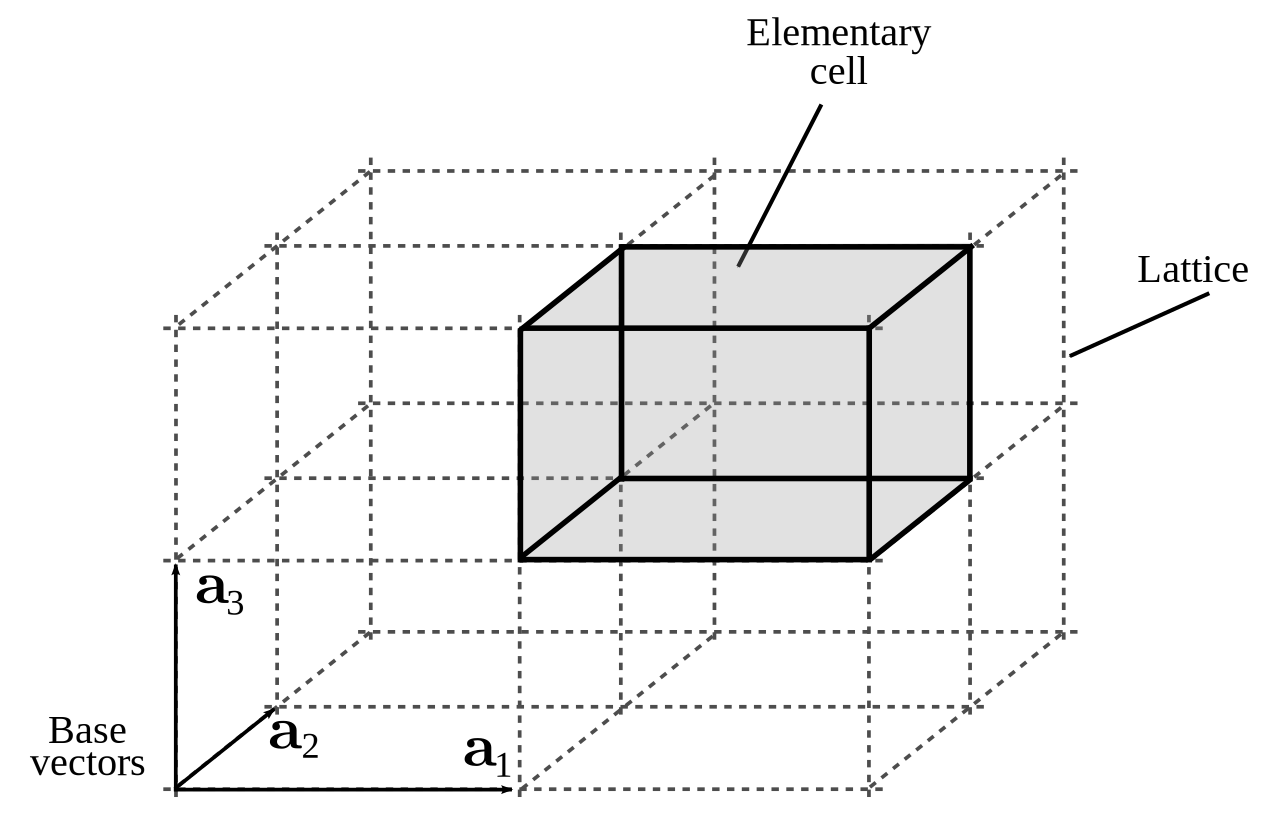
\includegraphics[height=8cm]{img/periodic_3D.pdf} 
\caption{Depiction of a periodic material in 3D.}
\label{fig:periodic_3D}
\end{figure}

\begin{figure}[h]
\centering
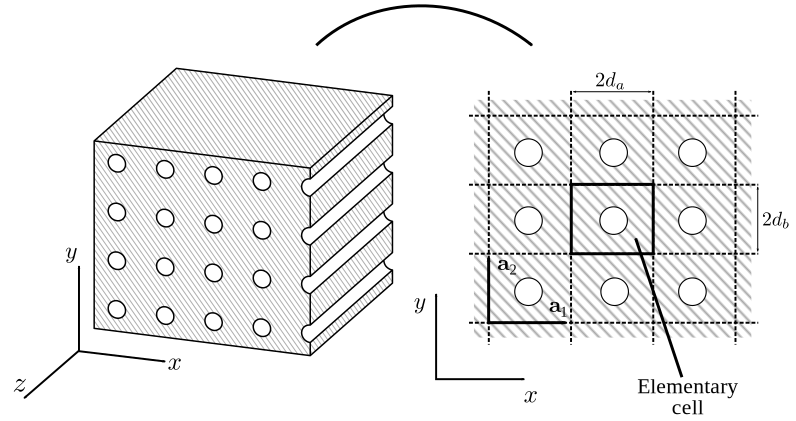
\includegraphics[height=8cm]{img/periodic_2D.pdf} 
\caption{Depiction of a periodic material in 2D.}
\label{fig:periodic_2D}
\end{figure}

\todo{Add Periodic media info.} Describe periodic boundary conditions and Bloch theorem as boundary conditions.

Periodic boundary conditions are common in molecular dynamics and micromechanics/homogenization.

\section{Bloch theorem}
Let us start from an equation of the form
\begin{equation}
 Lu(\mathbf{x}) = \omega^2 u(\mathbf{x}) \enspace ,
\label{eq:operator_eigenvalues}
\end{equation}
where $L$ is a differential operator with algebraic properties that are similar to the wave equation \cite{algebraic_waves}. The Bloch theorem establishes that the solution for  \eqref{eq:operator_eigenvalues} is given by
%
\begin{equation}
 u(\mathbf{x}) = w(\mathbf{x}) e^{i\mathbf{k}\cdot\mathbf{x}} \enspace ,
\label{eq:bloch_theorem}
\end{equation}
%
where $w(\mathbf{x})$ is function with the same periodicity of the material and is termed Bloch function. The theorem according to \cite{book:kittel1986} states
%
\begin{quote}
\emph{The eigenfunctions of the wave equation for a periodic potential are the product of a plane wave $\exp(i\mathbf{k}\cdot\mathbf{r})$ times a function $u_\mathbf{k}(\mathbf{r})$ with the periodicity of the crystal lattice.}
\end{quote}
%
If we write the solution \eqref{eq:bloch_theorem} for the point $\mathbf{x}+\mathbf{a}$, we obtain
\[
u(\mathbf{x} + \mathbf{a}) = w(\mathbf{x} + \mathbf{a}) e^{i\mathbf{k}\cdot(\mathbf{x} + \mathbf{a})} \enspace ,
\]
being $\mathbf{a} = n_i \mathbf{a}_i$ a vector with the periodicity of the lattice, and  $n_i \in \mathbb{Z}$. Since$w(\mathbf{x})$ should present the same periodicity of the lattice
\[
u(\mathbf{x} + \mathbf{a}) = w(\mathbf{x}) e^{i\mathbf{k}\cdot(\mathbf{x} + \mathbf{a})} \enspace ,
\]
implying
\[
w(\mathbf{x}) = u(\mathbf{x}+ \mathbf{a}) e^{-i\mathbf{k}\cdot(\mathbf{x} + \mathbf{a})} \enspace ,
\]
and substituting this in \eqref{eq:bloch_theorem}, we get
\begin{equation}
u(\mathbf{x} + \mathbf{a}) = u(\mathbf{x}) e^{i\mathbf{k}\cdot\mathbf{a}} \enspace .
\label{eq:bloch_theorem2}
\end{equation}
Equation \eqref{eq:bloch_theorem2} is termed Bloch periodicity or Bloch-periodic condition. Besides the form in equation \eqref{eq:operator_eigenvalues}, we can also have an equation of the form
\begin{equation}
 Lu(\mathbf{x}) = \omega^2 u(\mathbf{x})  + \mathbf{f}(\omega) \enspace ,
\end{equation}
where $\mathbf{f}(\omega)$ is a harmonic body force with circular frequency $\omega$ that presents the same periodicity that the lattice, see \cite{langlet-thesis}.

\section{Bloch analysis}

\section{Implementation}





